\section{Troca de Contexto Entre Máquinas Virtuais}

A troca de contexto refere-se ao processo de interromper a execução de uma máquina virtual em andamento,
salvando seu estado atual e restaurando o contexto de outra máquina virtual para que esta possa ser executada no processador.

Essa é uma das etapas mais críticas de um hipervisor, pois a corrupção do contexto de uma \gls{vm} pode praticamente inutilizá-la.

\subsection{RISC-V}

Para realizar essa operação na RISC-V, o processo foi dividido em duas etapas: a manipulação do contexto da CPU —
que inclui estruturas internas do próprio hipervisor associadas a cada \gls{vm} — e a manipulação do contexto no escopo da
máquina virtual, responsável por elementos específicos necessários ao \gls{so} convidado.

O contexto de CPU concentra-se no salvamento dos registradores gerais e dos  específicos do modo \textit{machine},
bem como na gestão em nível de \textit{Thread}, que constitui a unidade básica de execução do hipervisor.

Por sua vez, o contexto da \gls{vm} é responsável pelo salvamento de registradores que extrapolam o escopo do hipervisor,
incluindo os registradores do modo \textit{supervisor}, utilizados exclusivamente pelas \glspl{vm}.
Além disso, esse contexto gerencia a troca de espaços de endereçamento, a delegação de interrupções e a
invalidação do cache da \gls{mmu}.

\begin{figure}[h]
	\centering
	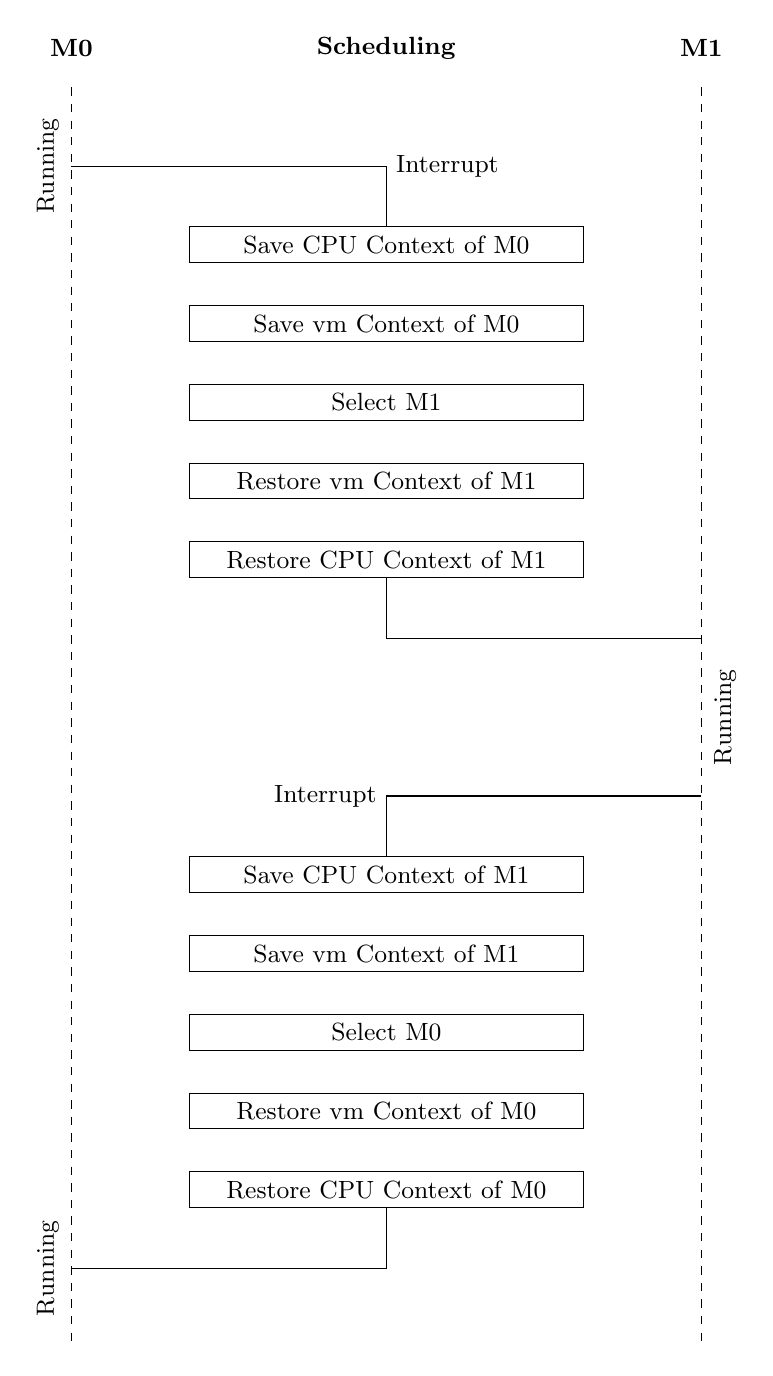
\begin{tikzpicture}[node distance=1.2cm, font=\small]
	
		\draw[dashed] (0,0) -- (0,-16);
		\draw[dashed] (8,0) -- (8,-16);
		\node at (0,0.5) {\textbf{M0}};
		\node at (8,0.5) {\textbf{M1}};

		\node at (4,0.5) {\textbf{Scheduling}};
		\node[rotate=90] at (-0.3,-1) {Running};
		\node[rotate=90] at (8.3,-8) {Running};
		\node[rotate=90] at (-0.3,-15) {Running};

		\node[draw, rectangle, minimum width=5cm] at (4, -2) (scpum0) {Save CPU Context of M0};
		\node[draw, rectangle, minimum width=5cm] at (4, -3) (svmm0) {Save \gls{vm} Context of M0};
		\node[draw, rectangle, minimum width=5cm] at (4, -4) (selectm1) {Select M1};
		\node[draw, rectangle, minimum width=5cm] at (4, -5) (rcpum1) {Restore \gls{vm} Context of M1};
		\node[draw, rectangle, minimum width=5cm] at (4, -6) (rvmm1) {Restore CPU Context of M1};

		\node[draw, rectangle, minimum width=5cm] at (4, -10) (scpum1) {Save CPU Context of M1};
		\node[draw, rectangle, minimum width=5cm] at (4, -11) (svmm1) {Save \gls{vm} Context of M1};
		\node[draw, rectangle, minimum width=5cm] at (4, -12) (selectm0) {Select M0};
		\node[draw, rectangle, minimum width=5cm] at (4, -13) (rcpum0) {Restore \gls{vm} Context of M0};
		\node[draw, rectangle, minimum width=5cm] at (4, -14) (rvmm0) {Restore CPU Context of M0};

		\draw (0,-1) -| node[right]{Interrupt} (scpum0.north);
		\draw (8,-7) -| (rvmm1.south);
		\draw (8,-9) -| node[left]{Interrupt} (scpum1.north);
		\draw (0,-15) -| (rvmm0.south);

	\end{tikzpicture}
	\caption{Troca de Contexto Entre Duas \Glspl{vm}}
\end{figure}
